% !TEX TS-program = pdflatex
% !TEX encoding = UTF-8 Unicode

% This is a simple template for a LaTeX document using the "article" class.
% See "book", "report", "letter" for other types of document.

\documentclass[11pt]{article} % use larger type; default would be 10pt

\usepackage[utf8]{inputenc} % set input encoding (not needed with XeLaTeX)
\usepackage{tikz}
%%% Examples of Article customizations
% These packages are optional, depending whether you want the features they provide.
% See the LaTeX Companion or other references for full information.

%%% PAGE DIMENSIONS
\usepackage{geometry} % to change the page dimensions
\geometry{a4paper} % or letterpaper (US) or a5paper or....
% \geometry{margins=2in} % for example, change the margins to 2 inches all round
% \geometry{landscape} % set up the page for landscape
%   read geometry.pdf for detailed page layout information

\usepackage{graphicx} % support the \includegraphics command and options

% \usepackage[parfill]{parskip} % Activate to begin paragraphs with an empty line rather than an indent

%%% PACKAGES
\usepackage{booktabs} % for much better looking tables
\usepackage{array} % for better arrays (eg matrices) in maths
\usepackage{paralist} % very flexible & customisable lists (eg. enumerate/itemize, etc.)
\usepackage{verbatim} % adds environment for commenting out blocks of text & for better verbatim
\usepackage{subfig} % make it possible to include more than one captioned figure/table in a single float
% These packages are all incorporated in the memoir class to one degree or another...
\usepackage{url}
\usepackage{hyperref}

%%% HEADERS & FOOTERS
\usepackage{fancyhdr} % This should be set AFTER setting up the page geometry
\pagestyle{fancy} % options: empty , plain , fancy
\renewcommand{\headrulewidth}{0pt} % customise the layout...
\lhead{}\chead{}\rhead{}
\lfoot{}\cfoot{\thepage}\rfoot{}

%%% SECTION TITLE APPEARANCE
\usepackage{sectsty}
\allsectionsfont{\sffamily\mdseries\upshape} % (See the fntguide.pdf for font help)
% (This matches ConTeXt defaults)

%%% ToC (table of contents) APPEARANCE
\usepackage[nottoc,notlof,notlot]{tocbibind} % Put the bibliography in the ToC
\usepackage[titles,subfigure]{tocloft} % Alter the style of the Table of Contents
\renewcommand{\cftsecfont}{\rmfamily\mdseries\upshape}
\renewcommand{\cftsecpagefont}{\rmfamily\mdseries\upshape} % No bold!

%%% END Article customizations

%%% The "real" document content comes below...

\usepackage{amsfonts}
\usepackage{amsmath}
\usepackage{amsthm}
\usepackage{amssymb}
\usepackage{wasysym}

\theoremstyle{definition}
\newtheorem*{beispiel}{Beispiel}
\newtheorem{definition}{Definition}
\newtheorem*{bemerkung}{Bemerkung}
\newtheorem*{beweis}{Beweis}
\newtheorem*{ubung}{Übung}

\title{Selbststudium 4}
\author{Florian Lüthi}
%\date{} % Activate to display a given date or no date (if empty),
         % otherwise the current date is printed 

\begin{document}
\maketitle

\section*{Aufgabe 2}

Beginnen wir mit Schritt 1:

\begin{center}
\begin{tabular}{r|c|c|c|c|c|c|c|}
\cline{2-2} $q_1$ & \\
\cline{2-3} $q_2$ && \\
\cline{2-4} $q_3$ &&&\\
\cline{2-5} $q_4$ &&&&\\
\cline{2-6} $q_5$ &&&&&\\
\cline{2-7} $q_6$ &&&&&&\\
\cline{2-8} $q_7$ &&&&&&&\\
\cline{2-8}		& $q_0$ & $q_1$ & $q_2$ & $q_3$ & $q_4$ & $q_5$ & $q_6$ 
\end{tabular}
\end{center}

Markieren wir als zweiten Schritt alle $\{s, t\}$ mit $s \notin F$ und $t \in F$:

\begin{center}
\begin{tabular}{r|c|c|c|c|c|c|c|}
\cline{2-2} $q_1$ & \\
\cline{2-3} $q_2$ && \\
\cline{2-4} $q_3$ &&&\\
\cline{2-5} $q_4$ &  &\smiley & \smiley & \smiley \\
\cline{2-6} $q_5$ &  & \smiley & \smiley & \smiley&\\
\cline{2-7} $q_6$ &&&&&&\\
\cline{2-8} $q_7$ &&&&&&&\\
\cline{2-8}		& $q_0$ & $q_1$ & $q_2$ & $q_3$ & $q_4$ & $q_5$ & $q_6$ 
\end{tabular}
\end{center}

Testen wir die Kombination als dritten Schritt:

\begin{center}
% Table generated by Excel2LaTeX from sheet 'Sheet2'
\begin{tabular}{rrrrrr}
\toprule
$s$   & $t$   & $\{\delta(s, 0), \delta(t, 0)\}$ &       & $\{\delta(s, 1), \delta(t, 1)\}$ &  \\
\midrule
$q_0$ & $q_1$ & $\{q_0,q_2\}$ &       & $\{q_1,q_3\}$ &  \\
$q_0$ & $q_2$ & $\{q_0, q_6\}$ &       & $\{q_1,q_2\}$ &  \\
$q_0$ & $q_3$ & $\{q_0, q_7\}$ &       & $\{q_1,q_2\}$ &  \\
$q_0$ & $q_4$ & $\{q_0, q_2\}$ &       & $\{q_1,q_4\}$ & \smiley \\
$q_0$ & $q_5$ & $\{q_0, q_3\}$ &       & $\{q_1,q_5\}$ & \smiley \\
$q_0$ & $q_6$ & $\{q_0, q_4\}$ &       & $\{q_1,q_7\}$ &  \\
$q_0$ & $q_7$ & $\{q_0, q_5\}$ &       & $\{q_1,q_7\}$ &  \\
$q_1$ & $q_2$ & $\{q_2,q_6\}$ &       & $\{q_3,q_2\}$ &  \\
$q_1$ & $q_3$ & $\{q_2,q_7\}$ &       & $\{q_3,q_2\}$ &  \\
$q_1$ & $q_6$ & $\{q_2,q_4\}$ & \smiley & $\{q_3,q_7\}$ &  \\
$q_1$ & $q_7$ & $\{q_2,q_5\}$ & \smiley & $\{q_3,q_7\}$ &  \\
$q_2$ & $q_3$ & $\{q_6, q_7\}$ &       & $\{q_2\} \notin \{s,t\}$ &  \\
$q_2$ & $q_6$ & $\{q_4, q_6\}$ &       & $\{q_2,q_7\}$ &  \\
$q_2$ & $q_7$ & $\{q_5, q_6\}$ &       & $\{q_2,q_7\}$ &  \\
$q_3$ & $q_6$ & $\{q_4, q_7\}$ &       & $\{q_2,q_7\}$ &  \\
$q_3$ & $q_7$ & $\{q_5, q_7\}$ &       & $\{q_2,q_7\}$ &  \\
$q_4$ & $q_5$ & $\{q_2, q_3\}$ &       & $\{q_4,q_5\}$ &  \\
$q_4$ & $q_6$ & $\{q_2, q_4\}$ & \smiley & $\{q_4,q_7\}$ &  \\
$q_4$ & $q_7$ & $\{q_2, q_5\}$ & \smiley & $\{q_4,q_7\}$ &  \\
$q_5$ & $q_6$ & $\{q_3, q_4\}$ & \smiley & $\{q_5,q_7\}$ &  \\
$q_5$ & $q_7$ & $\{q_3, q_5\}$ & \smiley & $\{q_5,q_7\}$ &  \\
$q_6$ & $q_7$ & $\{q_4, q_5\}$ &       & $\{q_7\} \notin \{s,t\}$  &  \\
\bottomrule
\end{tabular}%
\end{center}

Das führt uns zu:

\begin{center}
\begin{tabular}{r|c|c|c|c|c|c|c|}
\cline{2-2} $q_1$ & \\
\cline{2-3} $q_2$ && \\
\cline{2-4} $q_3$ &&&\\
\cline{2-5} $q_4$ & \smiley  &\smiley & \smiley & \smiley \\
\cline{2-6} $q_5$ &  \smiley & \smiley & \smiley & \smiley&\\
\cline{2-7} $q_6$ &&\smiley&&&\smiley&\smiley\\
\cline{2-8} $q_7$ &&\smiley&&&\smiley&\smiley&\\
\cline{2-8}		& $q_0$ & $q_1$ & $q_2$ & $q_3$ & $q_4$ & $q_5$ & $q_6$ 
\end{tabular}
\end{center}

Offensichtlich haben sich Markierungen geändert, also Schritt 3 von vorn:

\begin{center}
% Table generated by Excel2LaTeX from sheet 'Sheet2'
\begin{tabular}{rrrrrr}
\toprule
$s$   & $t$   & $\{\delta(s, 0), \delta(t, 0)\}$ &       & $\{\delta(s, 1), \delta(t, 1)\}$ &  \\
\midrule
$q_0$ & $q_1$ & $\{q_0,q_2\}$ &       & $\{q_1,q_3\}$ &  \\
$q_0$ & $q_2$ & $\{q_0, q_6\}$ &       & $\{q_1,q_2\}$ &  \\
$q_0$ & $q_3$ & $\{q_0, q_7\}$ &       & $\{q_1,q_2\}$ &  \\
$q_0$ & $q_6$ & $\{q_0, q_4\}$ & \smiley & $\{q_1,q_7\}$ & \smiley \\
$q_0$ & $q_7$ & $\{q_0, q_5\}$ & \smiley & $\{q_1,q_7\}$ & \smiley \\
$q_1$ & $q_2$ & $\{q_2,q_6\}$ &       & $\{q_3,q_2\}$ &  \\
$q_1$ & $q_3$ & $\{q_2,q_7\}$ &       & $\{q_3,q_2\}$ &  \\
$q_2$ & $q_3$ & $\{q_6, q_7\}$ &       & $\{q_2\} \notin \{s,t\}$ &  \\
$q_2$ & $q_6$ & $\{q_4, q_6\}$ & \smiley & $\{q_2,q_7\}$ &  \\
$q_2$ & $q_7$ & $\{q_5, q_6\}$ & \smiley & $\{q_2,q_7\}$ &  \\
$q_3$ & $q_6$ & $\{q_4, q_7\}$ & \smiley & $\{q_2,q_7\}$ &  \\
$q_3$ & $q_7$ & $\{q_5, q_7\}$ & \smiley & $\{q_2,q_7\}$ &  \\
$q_4$ & $q_5$ & $\{q_2, q_3\}$ &       & $\{q_4,q_5\}$ &  \\
$q_6$ & $q_7$ & $\{q_4, q_5\}$ &       & $\{q_7\} \notin \{s,t\}$  &  \\
\bottomrule
\end{tabular}%
\end{center}

Das führt uns zu:

\begin{center}
\begin{tabular}{r|c|c|c|c|c|c|c|}
\cline{2-2} $q_1$ & \\
\cline{2-3} $q_2$ && \\
\cline{2-4} $q_3$ &&&\\
\cline{2-5} $q_4$ & \smiley  &\smiley & \smiley & \smiley \\
\cline{2-6} $q_5$ &  \smiley & \smiley & \smiley & \smiley&\\
\cline{2-7} $q_6$ &\smiley&\smiley&\smiley&\smiley&\smiley&\smiley\\
\cline{2-8} $q_7$ &\smiley&\smiley&\smiley&\smiley&\smiley&\smiley&\\
\cline{2-8}		& $q_0$ & $q_1$ & $q_2$ & $q_3$ & $q_4$ & $q_5$ & $q_6$ 
\end{tabular}
\end{center}

Wiederum haben sich die Markierungen geändert -- da capo!

\begin{center}
% Table generated by Excel2LaTeX from sheet 'Sheet2'
\begin{tabular}{rrrrrr}
\toprule
$s$   & $t$   & $\{\delta(s, 0), \delta(t, 0)\}$ &       & $\{\delta(s, 1), \delta(t, 1)\}$ &  \\
\midrule
$q_0$ & $q_1$ & $\{q_0,q_2\}$ &       & $\{q_1,q_3\}$ &  \\
$q_0$ & $q_2$ & $\{q_0, q_6\}$ & \smiley & $\{q_1,q_2\}$ &  \\
$q_0$ & $q_3$ & $\{q_0, q_7\}$ & \smiley & $\{q_1,q_2\}$ &  \\
$q_1$ & $q_2$ & $\{q_2,q_6\}$ & \smiley & $\{q_3,q_2\}$ &  \\
$q_1$ & $q_3$ & $\{q_2,q_7\}$ & \smiley & $\{q_3,q_2\}$ &  \\
$q_2$ & $q_3$ & $\{q_6, q_7\}$ &       & $\{q_2\} \notin \{s,t\}$ &  \\
$q_4$ & $q_5$ & $\{q_2, q_3\}$ &       & $\{q_4,q_5\}$ &  \\
$q_6$ & $q_7$ & $\{q_4, q_5\}$ &       & $\{q_7\} \notin \{s,t\}$  &  \\
\bottomrule
\end{tabular}%
\end{center}

Das führt uns zu:

\begin{center}
\begin{tabular}{r|c|c|c|c|c|c|c|}
\cline{2-2} $q_1$ & \\
\cline{2-3} $q_2$ &\smiley&\smiley \\
\cline{2-4} $q_3$ &\smiley&\smiley&\\
\cline{2-5} $q_4$ & \smiley  &\smiley & \smiley & \smiley \\
\cline{2-6} $q_5$ &  \smiley & \smiley & \smiley & \smiley&\\
\cline{2-7} $q_6$ &\smiley&\smiley&\smiley&\smiley&\smiley&\smiley\\
\cline{2-8} $q_7$ &\smiley&\smiley&\smiley&\smiley&\smiley&\smiley&\\
\cline{2-8}		& $q_0$ & $q_1$ & $q_2$ & $q_3$ & $q_4$ & $q_5$ & $q_6$ 
\end{tabular}
\end{center}

Wir haben erneute Änderung der Markierungen festgestellt, also nochmal:

\begin{center}
% Table generated by Excel2LaTeX from sheet 'Sheet2'
\begin{tabular}{rrrrrr}
\toprule
$s$   & $t$   & $\{\delta(s, 0), \delta(t, 0)\}$ &       & $\{\delta(s, 1), \delta(t, 1)\}$ &  \\
\midrule
$q_0$ & $q_1$ & $\{q_0,q_2\}$ & \smiley & $\{q_1,q_3\}$ & \smiley \\
$q_2$ & $q_3$ & $\{q_6, q_7\}$ &       & $\{q_2\} \notin \{s,t\}$ &  \\
$q_4$ & $q_5$ & $\{q_2, q_3\}$ &       & $\{q_4,q_5\}$ &  \\
$q_6$ & $q_7$ & $\{q_4, q_5\}$ &       & $\{q_7\} \notin \{s,t\}$  &  \\
\bottomrule
\end{tabular}%
\end{center}

Das führt uns zu:

\begin{center}
\begin{tabular}{r|c|c|c|c|c|c|c|}
\cline{2-2} $q_1$ &\smiley \\
\cline{2-3} $q_2$ &\smiley&\smiley \\
\cline{2-4} $q_3$ &\smiley&\smiley&\\
\cline{2-5} $q_4$ & \smiley  &\smiley & \smiley & \smiley \\
\cline{2-6} $q_5$ &  \smiley & \smiley & \smiley & \smiley&\\
\cline{2-7} $q_6$ &\smiley&\smiley&\smiley&\smiley&\smiley&\smiley\\
\cline{2-8} $q_7$ &\smiley&\smiley&\smiley&\smiley&\smiley&\smiley&\\
\cline{2-8}		& $q_0$ & $q_1$ & $q_2$ & $q_3$ & $q_4$ & $q_5$ & $q_6$ 
\end{tabular}
\end{center}

Das einzig neu markierte Paar ist $\{q_0, q_1\}$, und dieses wird gemäss obiger Tabelle von nirgendwo her erreicht, also sind wir fertig mit Schritt 3.

In Schritt 5 bilden wir für jeden Zustand $s$ die Menge $S$:

\[
S_0 = \{q_0\}, S_1 = \{q_1\}, S_2 = \{q_2, q_3\}, S_4 = \{q_4, q_5\}, S_6 = \{q_6,q_7\},
\] ausserdem ist
\[
\Pi = \{S_0, S_1, S_2, S_4, S_6\}
\]
und
\[
F_\textrm{min} = \{ S \in \Pi | S \cap F \ne \varnothing \} = \{ S_0, S_4\}.
\]

Brauchen wir noch $\delta_\textrm{min}(S, a) = \bigcup\limits_{s \in S} \delta(s, a)$:

\begin{center}
% Table generated by Excel2LaTeX from sheet 'Sheet2'
\begin{tabular}{rrr}
\toprule
      & 0     & 1 \\
\midrule
$S_0$ & $\{q_0 \} \subseteq S_0$ & $\{q_1 \} \subseteq S_1$ \\
$S_1$ & $\{q_2 \} \subseteq S_2$ & $\{q_3 \} \subseteq S_2$ \\
$S_2$ & $\{q_6, q_7 \} \subseteq S_6$ & $\{q_2 \} \subseteq S_2$ \\
$S_4$ & $\{q_2, q_3 \} \subseteq S_2$ & $\{q_4, q_5 \} \subseteq S_4$ \\
$S_6$ & $\{q_4, q_5 \} \subseteq S_4$ & $\{q_7 \} \subseteq S_6$ \\
\bottomrule
\end{tabular}%
\end{center}

Nun sind wir endlich soweit, $A_\textrm{min} = (\Sigma, \Pi, \delta_\textrm{min}, S_0, F_\textrm{min})$ zeichnen zu können:

\begin{center}
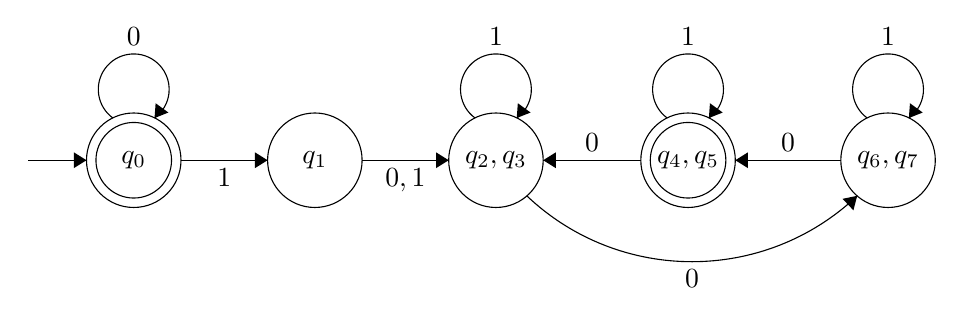
\begin{tikzpicture}[scale=0.2]
\tikzstyle{every node}+=[inner sep=0pt]
\draw [black] (10.2,-27.6) circle (3);
\draw (10.2,-27.6) node {$q_0$};
\draw [black] (10.2,-27.6) circle (2.4);
\draw [black] (21.7,-27.6) circle (3);
\draw (21.7,-27.6) node {$q_1$};
\draw [black] (33.2,-27.6) circle (3);
\draw (33.2,-27.6) node {$q_2,q_3$};
\draw [black] (45.4,-27.6) circle (3);
\draw (45.4,-27.6) node {$q_4,q_5$};
\draw [black] (45.4,-27.6) circle (2.4);
\draw [black] (58.1,-27.6) circle (3);
\draw (58.1,-27.6) node {$q_6,q_7$};
\draw [black] (3.5,-27.6) -- (7.2,-27.6);
\fill [black] (7.2,-27.6) -- (6.4,-27.1) -- (6.4,-28.1);
\draw [black] (8.877,-24.92) arc (234:-54:2.25);
\draw (10.2,-20.35) node [above] {$0$};
\fill [black] (11.52,-24.92) -- (12.4,-24.57) -- (11.59,-23.98);
\draw [black] (13.2,-27.6) -- (18.7,-27.6);
\fill [black] (18.7,-27.6) -- (17.9,-27.1) -- (17.9,-28.1);
\draw (15.95,-28.1) node [below] {$1$};
\draw [black] (24.7,-27.6) -- (30.2,-27.6);
\fill [black] (30.2,-27.6) -- (29.4,-27.1) -- (29.4,-28.1);
\draw (27.45,-28.1) node [below] {$0,1$};
\draw [black] (31.877,-24.92) arc (234:-54:2.25);
\draw (33.2,-20.35) node [above] {$1$};
\fill [black] (34.52,-24.92) -- (35.4,-24.57) -- (34.59,-23.98);
\draw [black] (56.139,-29.864) arc (-46.54553:-133.45447:15.25);
\fill [black] (56.14,-29.86) -- (55.21,-30.05) -- (55.9,-30.78);
\draw (45.65,-34.54) node [below] {$0$};
\draw [black] (42.4,-27.6) -- (36.2,-27.6);
\fill [black] (36.2,-27.6) -- (37,-28.1) -- (37,-27.1);
\draw (39.3,-27.1) node [above] {$0$};
\draw [black] (44.077,-24.92) arc (234:-54:2.25);
\draw (45.4,-20.35) node [above] {$1$};
\fill [black] (46.72,-24.92) -- (47.6,-24.57) -- (46.79,-23.98);
\draw [black] (56.777,-24.92) arc (234:-54:2.25);
\draw (58.1,-20.35) node [above] {$1$};
\fill [black] (59.42,-24.92) -- (60.3,-24.57) -- (59.49,-23.98);
\draw [black] (55.1,-27.6) -- (48.4,-27.6);
\fill [black] (48.4,-27.6) -- (49.2,-28.1) -- (49.2,-27.1);
\draw (51.75,-27.1) node [above] {$0$};
\end{tikzpicture}
\end{center}

Minimieren wir den bekannten Automaten $A$ noch mit dem zweiten vorgestellten Verfahren.

Bestimmen wir in Schritt 1:
\[
\Pi_1 = \{Q_{11}, Q_{12}\} = \{ F, Q-F\} = \{ \{q_0, q_4, q_5\}, \{q_1, q_2, q_3, q_6,q_7\}\}
\]

Bauen wir die Tabelle der Übergänge bezüglich $\Pi_1$:

\begin{center}
% Table generated by Excel2LaTeX from sheet 'Sheet3'
\begin{tabular}{r|rrr|rrrrr}
\toprule
      & \multicolumn{3}{c}{$Q_{11}$} & \multicolumn{5}{c}{$Q_{12}$} \\
      & $q_0$ & $q_4$ & $q_5$ & $q_1$ & $q_2$ & $q_3$ & $q_6$ & $q_7$ \\
\midrule
0     & $Q_{11}$ & $Q_{12}$ & $Q_{12}$ & $Q_{12}$ & $Q_{12}$ & $Q_{12}$ & $Q_{11}$ & $Q_{11}$ \\
1     & $Q_{12}$ & $Q_{11}$ & $Q_{11}$ & $Q_{12}$ & $Q_{12}$ & $Q_{12}$ & $Q_{12}$ & $Q_{12}$ \\
\bottomrule
\end{tabular}%
\end{center}

In Schritt 2 bilden wir gemäss der Bedingung die Partition $\Pi_2$:
\[
\Pi_2 = \{ \{q_0\}, \{q_4, q_5 \}, \{q_1, q_2, q_3 \}, \{q_6, q_7 \}  \} = \{ Q_{21}, Q_{22}, Q_{23}, Q_{24} \}
\]

Es gilt natürlich $\Pi_1 \ne \Pi_2$, also wiederholen wir den Schritt und bestimmen zuerst die Übergangstabelle bezüglich $\Pi_2$:

\begin{center}
% Table generated by Excel2LaTeX from sheet 'Sheet3'
\begin{tabular}{r|r|rr|rrr|rr}
\toprule
      & \multicolumn{1}{c}{$Q_{21}$} & \multicolumn{2}{c}{$Q_{22}$} & \multicolumn{3}{c}{$Q_{23}$}& \multicolumn{2}{c}{$Q_{24}$} \\
      & $q_0$ & $q_4$ & $q_5$ & $q_1$ & $q_2$ & $q_3$ & $q_6$ & $q_7$ \\
\midrule
0     & $Q_{21}$ & $Q_{23}$ & $Q_{23}$ & $Q_{23}$ & $Q_{24}$ & $Q_{24}$ & $Q_{22}$ & $Q_{22}$ \\
1     & $Q_{23}$ & $Q_{22}$ & $Q_{22}$ & $Q_{23}$ & $Q_{23}$ & $Q_{23}$ & $Q_{24}$ & $Q_{24}$ \\
\bottomrule
\end{tabular}%
\end{center}

Wir bilden die Partition $\Pi_3$ gemäss der Bedingung:
\[
\Pi_3 = \{\{q_0\}, \{ q_4,q_5\}, \{q_1\}, \{q_2, q_3\}, \{q_6, q_7\}\} = \{ Q_{31}, Q_{32}, Q_{33}, Q_{34}, Q_{35} \}
\]

Es gilt $\Pi_3 \ne \Pi_2$, also nochmal die Tabelle bezüglich $\Pi_3$:

\begin{center}
% Table generated by Excel2LaTeX from sheet 'Sheet3'
\begin{tabular}{r|r|rr|r|rr|rr}
\toprule
      & \multicolumn{1}{c}{$Q_{31}$} & \multicolumn{2}{c}{$Q_{32}$} & \multicolumn{1}{c}{$Q_{33}$}& \multicolumn{2}{c}{$Q_{34}$}& \multicolumn{2}{c}{$Q_{35}$} \\
      & $q_0$ & $q_4$ & $q_5$ & $q_1$ & $q_2$ & $q_3$ & $q_6$ & $q_7$ \\
\midrule
0     & $Q_{31}$ & $Q_{34}$ & $Q_{34}$ & $Q_{34}$ & $Q_{35}$ & $Q_{35}$ & $Q_{32}$ & $Q_{32}$ \\
1     & $Q_{33}$ & $Q_{32}$ & $Q_{32}$ & $Q_{34}$ & $Q_{34}$ & $Q_{34}$ & $Q_{35}$ & $Q_{35}$ \\
\bottomrule
\end{tabular}%
\end{center}

Wir bilden die Partition $\Pi_4$ gemäss der Bedingung:
\[
\Pi_4 = \{\{q_0\}, \{ q_4,q_5\}, \{q_1\}, \{q_2, q_3\}, \{q_6, q_7\}\} = \{ Q_{41}, Q_{42}, Q_{43}, Q_{44}, Q_{45} \}
\]

Es gilt $\Pi_4 = \Pi_3$, also sind wir fertig. Wir können nun $A_\textrm{min}$ bilden:

\[
A_\textrm{min} = (\Sigma, \Pi_4, \delta_{\Pi_4} = \delta_{\Pi_3}, Q_{31}, \{ Q_{31}, Q_{32} \})
\]

Und natürlich auch zeichnen:

\begin{center}
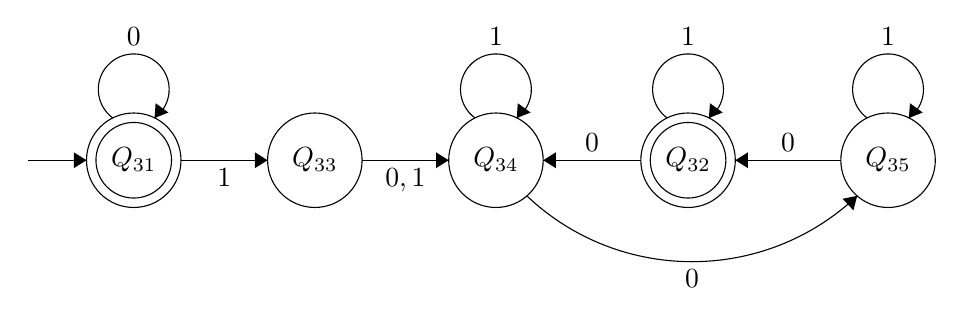
\begin{tikzpicture}[scale=0.2]
\tikzstyle{every node}+=[inner sep=0pt]
\draw [black] (10.2,-27.6) circle (3);
\draw (10.2,-27.6) node {$Q_{31}$};
\draw [black] (10.2,-27.6) circle (2.4);
\draw [black] (21.7,-27.6) circle (3);
\draw (21.7,-27.6) node {$Q_{33}$};
\draw [black] (33.2,-27.6) circle (3);
\draw (33.2,-27.6) node {$Q_{34}$};
\draw [black] (45.4,-27.6) circle (3);
\draw (45.4,-27.6) node {$Q_{32}$};
\draw [black] (45.4,-27.6) circle (2.4);
\draw [black] (58.1,-27.6) circle (3);
\draw (58.1,-27.6) node {$Q_{35}$};
\draw [black] (3.5,-27.6) -- (7.2,-27.6);
\fill [black] (7.2,-27.6) -- (6.4,-27.1) -- (6.4,-28.1);
\draw [black] (8.877,-24.92) arc (234:-54:2.25);
\draw (10.2,-20.35) node [above] {$0$};
\fill [black] (11.52,-24.92) -- (12.4,-24.57) -- (11.59,-23.98);
\draw [black] (13.2,-27.6) -- (18.7,-27.6);
\fill [black] (18.7,-27.6) -- (17.9,-27.1) -- (17.9,-28.1);
\draw (15.95,-28.1) node [below] {$1$};
\draw [black] (24.7,-27.6) -- (30.2,-27.6);
\fill [black] (30.2,-27.6) -- (29.4,-27.1) -- (29.4,-28.1);
\draw (27.45,-28.1) node [below] {$0,1$};
\draw [black] (31.877,-24.92) arc (234:-54:2.25);
\draw (33.2,-20.35) node [above] {$1$};
\fill [black] (34.52,-24.92) -- (35.4,-24.57) -- (34.59,-23.98);
\draw [black] (56.139,-29.864) arc (-46.54553:-133.45447:15.25);
\fill [black] (56.14,-29.86) -- (55.21,-30.05) -- (55.9,-30.78);
\draw (45.65,-34.54) node [below] {$0$};
\draw [black] (42.4,-27.6) -- (36.2,-27.6);
\fill [black] (36.2,-27.6) -- (37,-28.1) -- (37,-27.1);
\draw (39.3,-27.1) node [above] {$0$};
\draw [black] (44.077,-24.92) arc (234:-54:2.25);
\draw (45.4,-20.35) node [above] {$1$};
\fill [black] (46.72,-24.92) -- (47.6,-24.57) -- (46.79,-23.98);
\draw [black] (56.777,-24.92) arc (234:-54:2.25);
\draw (58.1,-20.35) node [above] {$1$};
\fill [black] (59.42,-24.92) -- (60.3,-24.57) -- (59.49,-23.98);
\draw [black] (55.1,-27.6) -- (48.4,-27.6);
\fill [black] (48.4,-27.6) -- (49.2,-28.1) -- (49.2,-27.1);
\draw (51.75,-27.1) node [above] {$0$};
\end{tikzpicture}
\end{center}

\end{document}
